 	 \section*{Introduction}
 	  
    Les Réseau de Pétri représentent un outil mathématique puisant dans le domaine de la modélisation et de la vérification des systèmes. En plus de leur force d’analyse, ils offrent une représentation graphique simple qui aide à la modélisation des systèmes complexes. 
    
    Donc Le modèle des réseaux de Pétri est un outil graphique de modélisation et d'analyse des systèmes parfaitement adapté à l'étude des structures de contrôle. Il permet notamment de maîtriser et d'assurer la sûreté de fonctionnement de logiciels complexes (aéronautique, transports, industrie...). 
    
    Le formalisme formel des Réseau de Pétri (RdP), adapté à la prise en compte des problèmes de concurrence, de synchronisme et de parallélisme, constitue un excellent outil de spécification fonctionnelle d'un problème et de mise en évidence des contraintes. Les propriétés mathématiques qui découlent de l'analyse des RdPs permettent une étude comportementale et structurelle essentielle à la validation d'une spécification. Les possibilités de simulation offertes par les outils informatiques supportant le formalisme contribuent également à cette validation. 
    
    En général, les méthodes de l'étude de systèmes par réseau de pétri se composent de trois étapes : premièrement on écrit le système en termes de réseau, pour obtenir un modèle en réseau ; deuxièmement on analyse le modèle obtenu, pour en déduire des propriétés comme l’absence de blocage, existence d'une solution, etc. Finalement, on fait la révision des propriétés obtenues pour montrer si le système est bon. Le résultat de cette méthode nous indique une analyse qualitative du système. Elle constitue une approche très importante pour avoir une bonne évaluation des systèmes.
    
    
 %La modélisation par les processus dont les domaines d'application étaient relativement restreints à l'origine, n'a cessé de progresser. Elle s'impose, aujourd'hui, en tant qu'outil incontournable, placé au cœur de la gestion des organisations. La déclinaison des processus organisationnels au niveau des architectures logicielles a donné, entre autres, naissance au workflow afin de répondre à des besoins divers dont celui d'optimisation des processus opérationnels, support et de pilotage.
%
%\section{Modélisation des processus workflow
%}
%La modélisation est une activité qui précède toute décision ou formulation, elle permet de représenter la description du système réel. Tout comme un système informatique, le système workflow comporte un certain nombre d'aspects à modéliser. Nous présentons en premier lieu ces aspects, nous décrivons en second lieu les principales techniques de modélisation utilisées dans le domaine de workflow et nous terminons cette section par évoquer certains aspects temporels et organisationnels des workflows.
%
%\subsection{Aspects à modéliser}
%\subsubsection{L'aspect fonctionnel}
%L'aspect fonctionnel concerne l'identification des activités des processus que l'on souhaite modéliser. Il est important de comprendre qu'il ne s'agit pas uniquement d'identifier les fonctions des différents départements d'une organisation mais aussi de distinguer les activités composant un processus. La modélisation fonctionnelle doit également permettre d'établir la hiérarchie des activités, i.e. d'exprimer de possibles décompositions en termes de sous-processus. 
%
%Enfin, le modèle fonctionnel doit aussi représenter le flux de données associées aux activités et les interdépendances de données entre les activités (data flow). 
%\subsubsection{L'aspect comportemental}
%L'aspect comportemental est un aspect primordial du workflow puisqu'il correspond à la dynamique du processus. Le comportement s'exprime par la modélisation d'un contrôle de flux entre les activités. Ce dernier permet d'indiquer la chronologie de l'exécution des activités, leur flux (séquentiel ou parallèle), les points de synchronisation entre activités ou au contraire, les points de disjonction. De plus, le modèle comportemental doit représenter les événements qui permettent de déclencher les activités. Nous soulignons l'importance de ce modèle, qui permet l'exécution du workflow. L'aspect comportemental est également appelé aspect de coordination.
%\subsubsection{ L'aspect informationnel (données) }
%Cet aspect concerne l'ensemble des informations et des données qui sont associées
%aux activités. Le modèle informationnel, souvent négligé lors de l'implémentation d'un workflow \parencite{b3}, décrit en détail les relations qui existent entre les données, leur type et leur structure.
%\subsubsection{L'aspect organisationnel }
%Comme son nom l'indique, la partie organisationnelle concerne la description de l'organisation des acteurs de l'entreprise. Le modèle organisationnel peut soit refléter fidèlement l'organigramme de l'entreprise, c'est à dire la décomposition hiérarchique de celle-ci en départements et services soit décrire des unités organisationnelles dans lesquelles on identifie des acteurs. Selon la méthode choisie, la description est plus ou moins détaillée et permet d'établir des liens hiérarchiques entre les acteurs ainsi que des relations entre unités organisationnelles ou départements. Toutefois, quelle que soit la méthode retenue, la description des rôles associés aux différentes activités reste invariante. Les rôles créent l'interface entre le modèle organisationnel et les modèles représentant les activités.
%
%
%
%\subsection{Modélisation de Workflow adaptable }
%
%Dans le cas particulier de la modélisation des Workflow adaptables, plusieurs approches sont proposées [HAN 98]. 
%
%\subsubsection{ Approche Meta modèle}
%Cette approche emploie un méta modèle pour déterminer la structure et les types de composants constitutifs; elle définit un jeu de primitives pour transformer un modèle Workflow générique ou une instance de modèle. 
%
%\subsubsection{ L’approche de point ouvert Open-point }
%Elle définit des points spéciaux dans un modèle de Workflow, où l’adaptation peut être faite. Cette approche inclut la mise à disposition de choix multiples pour les utilisateurs, l’allocation dynamique de certaines ressources aux tâches en run time, ou une interface ouverte par laquelle une « dernière modélisation » peut être réalisée. La « dernière modélisation » signifie que, pendant l’exécution des modèles complets, certains sous modèles peuvent être définis dynamiquement pour une utilisation immédiate. 
%\subsubsection{ Approche synthétisée}
%Il semble que les deux approches puissent être employées complémentairement pour la définition de Workflow adaptable. Pour cela, les deux hypothèses suivantes doivent être prises en compte :
%
%Tout d’abord, il parait nécessaire de distinguer les évolutions de procédures Workflow et les changements ad hoc dynamique dans une procédure. De plus, une séparation claire est faite entre le build time et le run time en termes de Workflow. Il parait impératif de faciliter le franchissement bilatéral de cette frontière pour rendre modélisables les Workflow adaptables.
%
%En synthèse, il est souhaitable de définir la frontière entre les changements ad hoc et les évolutions du Workflow. Il semblerait que ces changements devraient être testés sur une instance de modèles puis si nécessaires propagés au niveau global pour une modification persistante.


\section{Réseau de Pétri}

\subsection{Qu'est-ce que les réseaux de Pétri }
Les réseaux de Pétri sont définis comme étant un formalisme qui permet la description et l'analyse du comportement des systèmes concurrents, introduit par Carl Adam Pétri en 1962. [1]  Les définitions concernant les réseaux de Pétri portaient sur deux aspects :


\begin{itemize}
	\item \textbf{	Un aspect structurel }
\\
	Quelles sont les actions, quels sont les sites, quelles sont les conditions pour qu'une action soit possible et quelles sont les conséquences d'une action?
	
	\item \textbf{ Un aspect comportemental}
	\\
	Comment représenter le fonctionnement d'un réseau de Pétri? C.-à-d. ce qui se passe quand une action ou plusieurs actions sont exécutées.
\end{itemize}

\subsection{L'aspect structurel}
\begin{defn}\textbf{\textbf{(Définition d'un réseau de pétri:}}
	\\
Un réseau de pétri (R) est un triple R= (P, T, W) où P est l'ensemble des places (les places représentent les sites) et T l'ensemble des transitions (les transitions représentent les actions) tel que :
	
	\begin{itemize}
		\item  	P est un ensemble final de places,
		\item T est un ensemble final de transition $ (P \cap T = \theta ) $ ,
		\item W: $(P \times T) \cup (T \times P)\to N = \{0,1,2,...\} $  .
	\end{itemize}
	
\end{defn}

\subsubsection{Représentation d'un réseau de Pétri }


 
 \subsubsection*{Représentation graphique} 
  L'un des aspects les plus agréables des réseaux de Pétri est qu'il est extrêmement aisé de les visualiser; c.-à-d., donner une interprétation graphique à sa structure qui peut être représentée à travers un graphe bipartie fait de deux types de sommets: les places et les transitions reliées alternativement par des arcs orientés qui portent des poids entiers positifs, si un poids n'est pas porté alors il est égal à 1 (RdP ordinaire). Généralement, les places sont représentées par des cercles et les transitions par des rectangles, le marquage d'un RdP est représenté par la distribution de jetons dans l'ensemble de ses places telle que chaque place peut contenir un ou plusieurs jetons représentés par des points dans le cercle représentant la place. [2]
 
 
 
\begin{figure}[h]
	\centering
	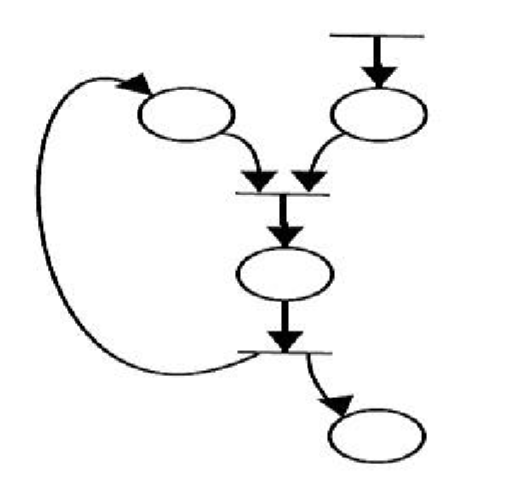
\includegraphics[width=0.5\linewidth]{images/petrif01}
	\caption{ Réseau de Pétri simple }
	\label{fig:petrif01}
\end{figure}
 	 \subsubsection*{ Représentation matricielle} 
 	Une représentation matricielle d'un RdP est offerte afin de simplifier les Tâches d'analyse et de vérification effectuée sur un modèle RdP. Agir sur une représentation graphique d'un modèle RdP est une Tâche délicate en comparant avec une représentation matricielle. Il   est possible de représenter la fonction W (fonction de poids) par des matrices.[2] 
  
  \begin{defn}\textbf{\textbf{(Réseau de pétri):}}
  	Soit Un réseau de pétri $ R= (P, T, W) $ avec $ P= \{p1, p2, …, pm\} $ et $ T= \{t1, t2, …,tn \}$, on appelle matrice des pré conditions   pré la matrice  $  m \times n $   à coefficients dans  N  tel que $ pre (i,j)= W(p_{i}, t_{j}) $ , elle indique le nombre de marques que doit contenir la place $p_{i}$ pour que la transition $ tj $  devienne franchissable, de la même manière on définit la matrice des post conditions post  la matrice $ n  \times m $ tel que $ post (i,j)= W(tj,  p_{i}) $ contient le nombre de   marques déposées dans $p_{i}$ lors du franchissement de la transition $t_{j}$. La matrice C= post – pré est appelée matrice d'incidence du réseau (m représente le nombre de places d'un réseau de Pétri et n le nombre de transitions.). 
  \end{defn}

La représentation Graphique d’un marquage dans un RdP marqué est présentée par des marques dans la place appelées jetons. 

Le marquage d'un réseau de Petri est représenté par un vecteur de dimension m à coefficients dans N. La règle de franchissement d'un réseau de Petri est définie par :    $     M’ (p) =M (p) +  C (p, t).  $
  
  
  
  \subsubsection*{Représentation d’un RdP marqué }

Un réseau de Pétri marqué est le couple $ N = < R , M > $ où : 
\begin{itemize}
	\item R est un réseau de Pétri .
		\item M est une application de marquage  .
		\item $  M : P \to N  $ .
\end{itemize}


$ M(p) $ est le nombre de marques (jetons) contenus dans la place p. Le marquage d’un réseau de Pétri est une opération qui consiste à assigner des jetons dans les places.

On appelle marquage M d’un Réseau de Pétri le vecteur du nombre de marques dans chaque place : la $ I^{eme} $ composante  correspond au nombre de marques dans la $ I^{eme} $   place. Il indique à un instant donné l'état du RdP.[2]   


\begin{exmp}
 

\begin{figure}[H]
	\centering
	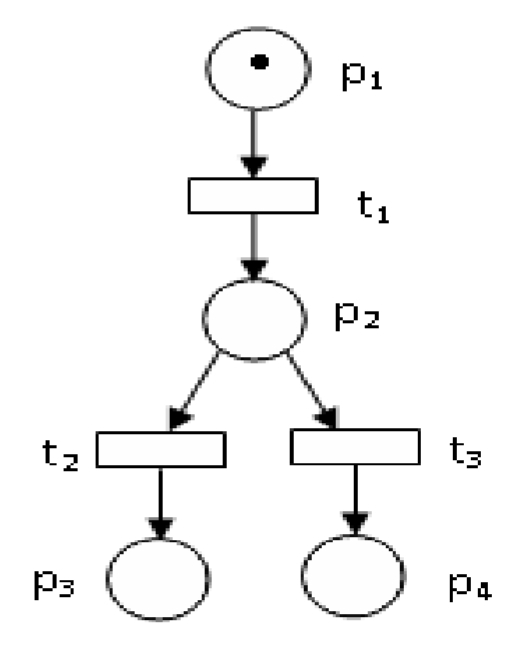
\includegraphics[width=0.4\linewidth]{images/pitref02PNG}
	\caption{ Réseau de Pétri marqué }
	\label{fig:pitref02png}
\end{figure}

Pour le réseau de la (Figure \ref{fig:pitref02png}) .

$ P= \{p1, p2, p3, p4\}$ et $T= \{t1, t2, t3\}  $

 
 \begin{figure}[H]
 	\centering
 	
 	\begin{subfigure}[b]{0.4\textwidth}
 	 \[
 	 pre=
 	 \begin{pmatrix}
 	 1 & 0 & 0 \\
 	 0 & 1 & 1 \\
 	 0 & 0 & 0 \\
 	 0 & 0 & 0
 	 \end{pmatrix}
 	 \]
 	  		\caption{La matrice pré}
 	\end{subfigure}
 	\hfill
 	\begin{subfigure}[b]{0.4\textwidth}
 \[	post=
 	\begin{pmatrix}
 		1 & 0 & 0 \\
 		0 & 1 & 1 \\
 		0 & 1 & 1 \\
 		0 & 0 & 0 
 	\end{pmatrix}
 	\]
 		\caption{La matrice post}
 	\end{subfigure}
 

	
	\begin{subfigure}[b]{0.4\textwidth}
		\[
		C=
		\begin{pmatrix}
		-1 & 0 & 0 \\
		0 & -1 & -1 \\
		0 & 1 & 0 \\
		0 & 0 & 1
		\end{pmatrix}
		\]
			\caption{La matrice d'incidence}
	\end{subfigure}
	\hfill
	\begin{subfigure}[b]{0.4\textwidth}
		\[	M=
		\begin{pmatrix}
		1  \\
		0  \\
		0  \\
		0 
		\end{pmatrix}
		\]
			\caption{Le vecteur de marquage M }
	\end{subfigure}
	
\end{figure}

Le marquage du RdP présenté à la Figure 3 est donné par : 
	\[	M=
\begin{pmatrix}
1  \\
0  \\
0  \\
0 
\end{pmatrix}
\]
On appelle marquage initial, noté M0, le marquage à l’ instant initial (t = 0). 
\end{exmp}
 

\subsection{ L'aspect comportemental }

Le comportement d'un réseau de Pétri est déterminé par sa structure et par son état. Pour exprimer l'état d'un réseau de Pétri, les places peuvent contenir des jetons qui ne sont que de simples marqueurs. .[1] 
\subsubsection{L’état dans un réseau de Pétri  }
Dans la théorie des réseaux de Pétri, l'état d'un réseau est souvent appelé marquage du réseau qui est définit par la distribution des jetons sur les places. Le marquage d'un réseau   de 
Pétri $ R= (P, T, W) $ est défini par la fonction de marquage $  M : P \to N $. 

Un réseau de Pétri marqué est dénoté par $ \sum = (P, T, W, M_{0}) $ où $M_{0}$ est le marquage initial. Le comportement d'un réseau de Pétri marqué est déterminé par ce qu'on appelle règle de franchissement. 

\subsubsection{ Franchissement d’une transition }
Une règle de franchissement est une simple relation de transition qui définit le changement d'état dans un réseau marqué lors de l'exécution d'une action. Afin de définir une règle de franchissement, il est nécessaire de formaliser quand le réseau peut exécuter une action:  on  dit  qu'une  transition $t \in T$ peut  être  franchie  à  partir  d'un  marquage  M  (qui représente l'état du système à un instant donné) si et seulement si chaque place d'entrée $p  \in$$^{*}t$ de la transition t contient au moins un nombre de jetons qui est supérieur ou égal au poids de l'arc reliant cette place d'entrée p avec la transition t  tel que:   $M(p)   \geq W(p, t)  \forall p \in P$. Une règle de franchissement est définie par $M'(p) = M (p) - W(p, t) + W(t, p)$ pour  tout $p \in P$, ce qui veut dire que lorsque la transition t est franchie à partir d'un marquage M, il faut saisir  W(p, t) jetons à partir de chaque place d'entrée à la transition t et déposer W(t, p) jetons dans chaque place de sortie de la transition t ce qui permet de produire un nouveau marquage M'. 

Le franchissement d'une transition t dénoté par $M[t > M' $est dite l'occurrence de t. On  dit que deux transitions t1, t2  (pas nécessairement distinctes) sont franchies en concurrence par un marquage M  si et seulement si $ M (p) \geq W(p, t_{1}) + W(p, t_{2})$ pour toute $p \in P$. .[3] 

Cette vision de l'exécution concurrente de deux transitions dans un RdP est contradictoire avec celle qui impose que deux occurrences de transition sont parallèles si et seulement si : elles sont causalement indépendantes et n'ont pas une relation de conflit entre eux. Deux occurrences sont en conflit si l'un des deux peut avoir lieu mais pas toutes les deux.


\subsubsection{L'exécution d'un réseau de Pétri }

\subsubsection*{Exécution séquentielle }
\begin{enumerate}
\item \textbf{Séquence de franchissement:}
 Une séquence de franchissement « s » est une suite de transitions (t1, t2, …, tn) qui permet, à partir d’un marquage « M », de passer au marquage « M’ » par le franchissement successif des transitions définissant la séquence.
  \item \textbf{Marquage accessible :}Le marquage d’un Réseau de Pétri à un instant donné est une vectrice colonne dont la valeur de la Ième composante est le nombre de marques dans la place $P_{i}$ à cet instant.
  
  
  
  Le franchissement d’une transition conduit à un changement du marquage. Le passage du marquage $M_{k}$ au marquage $M_{l}$ par franchissement de la transition $T_{j}$ est noté :$ M_{k} (T_{j } > M_{l}$. Le nombre de marques dans la place $P_{i}$ pour le marquage Mk est noté $M_{k}(P_{i})$. A partir d’un Même marquage, il peut être possible de franchir plusieurs transitions, menant ainsi à des marquages différents. L’ensemble des marquages accessibles à partir du marquage $M_{0}$ est l’ensemble des marquages obtenus à partir de $ M_{0}$ par franchissements successifs d’une ou plusieurs transition(s). Cet ensemble est noté $ A(R ; M_{0})$. [3]  
  
  \item  \textbf{Graphe de marquage :}
  On peut représenter l’ensemble des marquages accessibles par un graphe si ce dernier et fini. Le graphe de marquage  a comme sommet l’ensemble des marquages accessibles $A(R,M_{0})$. Un arc orienté relie deux sommet $M_{i}$ et $M_{j}$ s’il existe une transition t franchissable permettant de passer d’un marquage à un autre $M_{i} [t>M_{j}$ . Les arcs du graphe sont étiquetés par les transitions correspondantes. [3] 
  
  
  \begin{exmp}
   \end{exmp}
\begin{figure}[H]
	\centering
	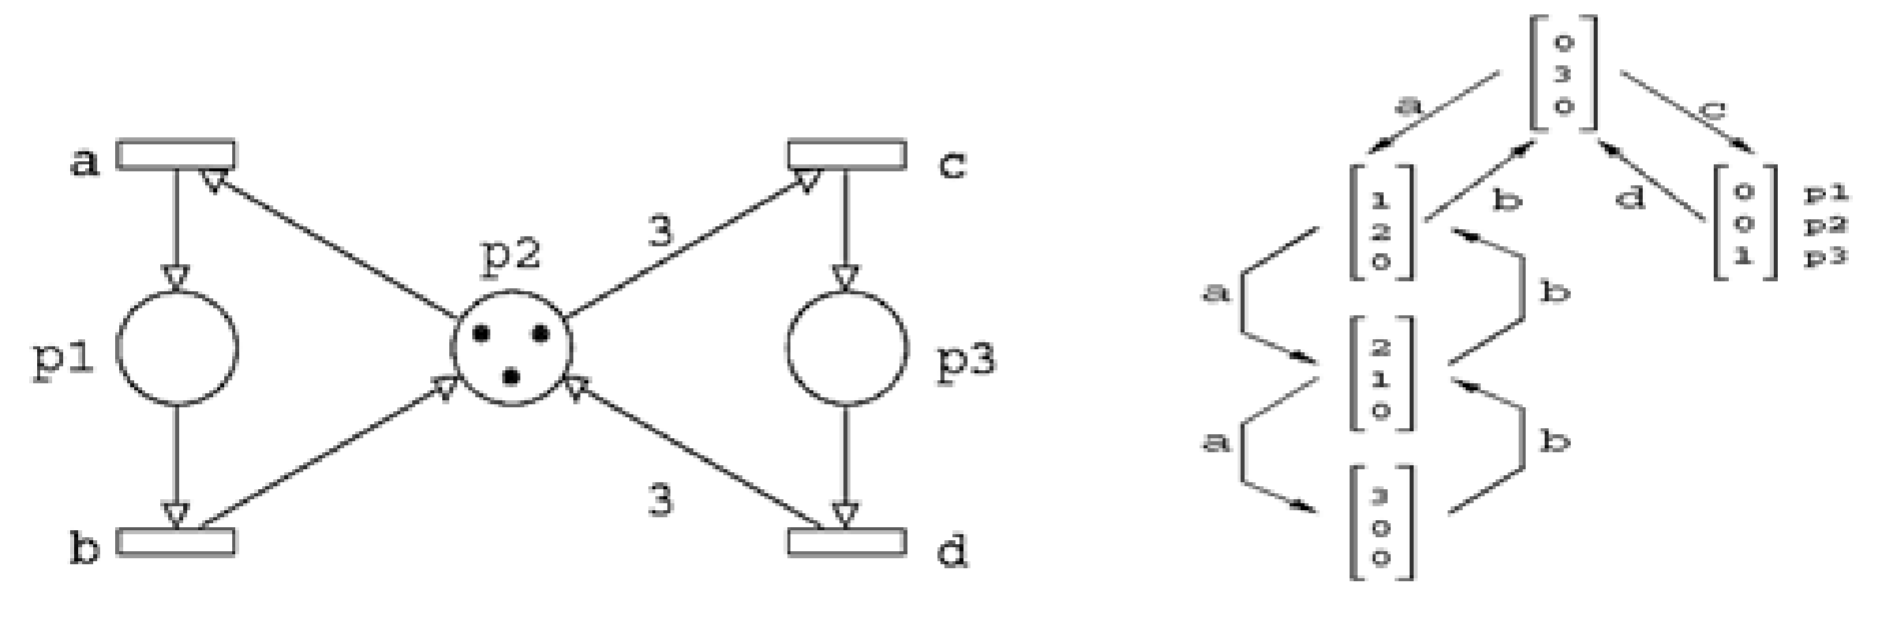
\includegraphics[width=1\linewidth]{images/pitrif03}
	\caption{Graphe de Marquage }
	\label{fig:pitrif03}
\end{figure}

  
  \item \textbf{L'exécution séquentielle d'un réseau de Pétri }
  
  L'exécution séquentielle d'un réseau de Pétri est définie en termes d'un ensemble de séquences d'occurrences. Une séquence d'occurrences est une séquence de transitions franchissables dénotée par $ \sigma =M_{0} t_{1} M_{1} t_{2}…$tel que $M_{i-1}[t_{i} > M_{i}$. Une séquence$ t_{1} t_{2}…$ est une séquence de transitions (commencée par le marquage M) si et seulement si il existe une séquence d'occurrences M0t1M1... avec $M=M_{0}$. Si la séquence finie $t_{1} t_{2}…t_{n}$ conduit à un nouveau marquage M' à partir du marquage M, on écrit $M[t_{1} t_{2}…t_{n} > M’$ ou simplement $M[t_{1} t_{2}…t_{n} >  si $ on ne veut pas spécifier le marquage résultat. [3] 
  
  
  
  
  
\end{enumerate}



\subsubsection*{Exécution concurrente }


Une exécution concurrente d'un réseau de Pétri est une exécution dans laquelle  plusieurs transitions peuvent se franchir en même temps, elle est souvent déterminée par la notion de processus. Ceci permet de donner une interprétation de la concurrence dans un réseau de Petri selon la sémantique basée sur la vraie concurrence (sémantique d'ordre partiel) qui est interprétée dans la théorie des réseaux de Pétri par un type spécial de réseaux appelés réseaux d'occurrences. [3] 



 \section{Réseaux particuliers }



\section{Propriétés des réseaux de Petri}
il existe un certain nombre de propriétés qui ont été définis pour les réseaux de Petri, à savoir, le caractère borné, la réinitilisation la vivacité , la conservation, la terminaison (Diaz, 2001). Certaines de ces propriétés sont dites propriétés dynamiques car elles dépendent du marquage initial et sont liées à l'évolution du réseau,alors que d'autres sont dites propriétés statiques du fait qu'elles soient liées à la typologie du réseau et indépendantes du marquage initial.

\subsection{Réseau K-borné }
\begin{defn}\textbf{\textbf{(Réseau de Petri borné):}}\\
	Une place $ P_{i} $ est bornée pour un marquage initial $ M_{0} $ si pour tout marquage accessible à partir de $ M_{0} $, le nombre de jetons dans $P_{i}$ reste borné. Elle est dite k-bornée si le nombre de jetons dans $ P_{i} $ est toujours inférieur ou égal à k. Un RdP est(k) borné si tout esses places sont(k)bornées.
	
\end{defn}

\begin{exmp}
	Un RdP peut ne pas être borné. Sur l'exemple représenté à la (figure \ref{fig:rdpborn}), la transition $ T_{1} $ admet la place $ P_{1} $ comme unique place d'entrée.La place P1 a un jeton:la transition $ T_{1} $
\end{exmp}

\begin{figure}[h]
	\centering
	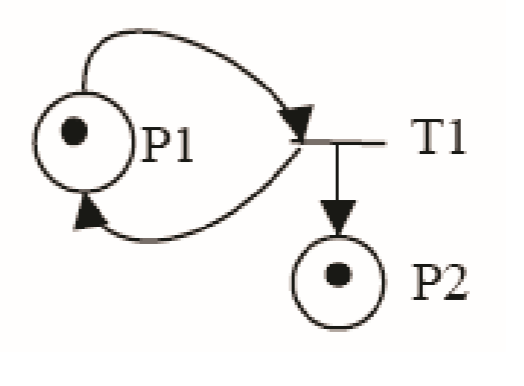
\includegraphics[width=0.5\linewidth]{images/Rdpborn}
	\caption{Réseau de Petri non borné}
	\label{fig:rdpborn}
\end{figure}

est franchissable. Comme $ P_{1} $ est aussi place de sortie de $ T_{1} $,le franchissement de $ T_{1} $ ne change pas le marquage de $ P_{1} $.La transition $ T_{1} $ est donc franchissable en permanence et peut donc être franchie un nombre de fois infini.Chaque franchissement de $ T_{1} $ ajoute un jeton dans $ P_{2} $ dont le marquage va donc tendre vers l'infini.

\begin{defn}\textbf{Réseau de Petri sauf:}\\
	Un RdP est sauf ou binaire pour un marquage initial M0 s'il est un borné.
	
\end{defn}

\subsection{Réseau vivant }
\begin{defn}\textbf{La vivacité:}\\
	Une transition $ T_{j} $ est vivante pour un marquage initial $ M_{0} $ si pour tout marquage accessible $ M_{k} $ , il existe une séquence de franchissement $ S $ à partir de $ M_{k} $ contenant $T_{j}: M_{k} \in^{*} M_{0},   \exists S,M_{k}| S>$ et $S = ... T_{j} ...$
	\\
	
	Si une transition $ T_{j} $ est vivante alors, à tout instant, on sait que $ T_{j} $ peut être franchie dans le futur. Dans le cas d'un réseau de Petri modélisant un système fonctionnant en permanence, si une transition n'est pas vivante et si une fonction du système est associée au franchissement de cette transition,ce la veut dire qu'à partir d’un certain instant ,cette fonction ne sera plus disponible dans le futur, ce qui peut traduire une erreur ou une panne.
	
\end{defn}

\begin{figure}[H]
	\centering
	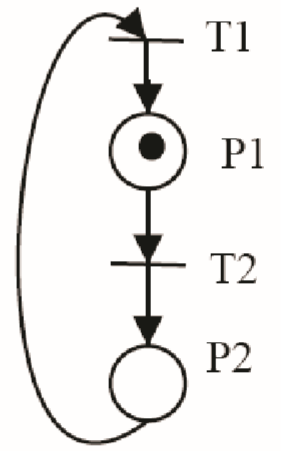
\includegraphics[width=0.2\linewidth]{images/Petrivivant}
	\caption{Réseau de Petri vivant}
	\label{fig:petrivivant}
\end{figure}

\begin{defn}\textbf{Blocage:}\\
	Un blocage (ou état puits)est un marquage pour lequel aucune transition n'est validée.
\end{defn}


Un réseau de Petri est dit sans blocage pour un marquage initial $M_{0}$ si aucun marquage accessible n'est un blocage.

\begin{figure}[H]
	\centering
	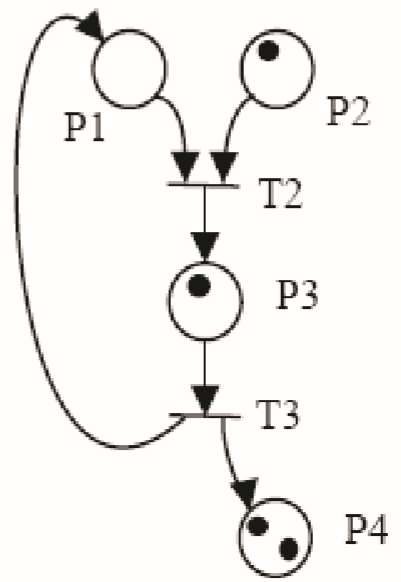
\includegraphics[width=0.25\linewidth]{images/Petribloquant}
	\caption{Exemple de réseau de Petri bloquant}
	\label{fig:petribloquant}
\end{figure}

Le réseau de Petri de la (Figure \ref{fig:petribloquant}), par exemple ,a pour blocage le marquage: 
$M = (1,0,0,1)$.

\subsection{Réseau réinitialisable }
\begin{defn} \textbf{(états d' accueil et Réseau de Petri réinitialisable ) }\\
	Un RdP a un état d’accueil $ M_{a} $ pour un marquage initial $ M_{0} $ si pour tout marquage accessible $ M_{k} $ à partir de $ M_{0} $, il existe une séquence de franchissement permettant d'atteindre le marquage
	$M_{a}: \forall M_{k} \in^{*} M_{0},   \exists S_{j},M_{k}|S_{j}>M_{a}$
\end{defn}
Un RdP est réinitialisable pour un marquage initial $ M_{0} $ si $ M_{0} $ est un\\
état d'accueil.
\\

Si un réseau de Petri présente un état d’accueil, il est facile de vérifier s’il est sans blocage et d'étudier sa vivacité.

\section{ Réseaux de Pétri de haut niveau }
Dans la pratique, on est amené à modéliser toute sorte de système, à savoir les protocoles de communication, les systèmes de production, les systèmes réactifs, les systèmes temps réel, etc. Cette variété de systèmes a poussé les chercheurs à étendre la théorie des RdPs en introduisant beaucoup de concepts relatifs à chaque domaine d’application. Ces efforts ont donné naissance aux RDPs de haut niveau tels que les RDPs colorés, hiérarchiques, temporisés et autres. [6] 
\subsection{Les réseaux de Petri colorés}
Les réseaux colorés(Jensen, 1997)ont été introduits afin de modéliser des systèmes complexes tout en gardant les possibilités de vérification. Lorsque le nombre d'entités du système à modéliser est important,la taille du réseau de Petri devient rapidement énorme,et si les entités présentent des comportements similaires, l'usage des réseaux colorés permet de condenser le modèle. En effet, une couleur est une information attachée à un jeton. Cette information permet de distinguer des jetons entre eux et peut être de type quelconque. Par conséquent, une place peut contenir des jetons de différentes couleurs et une transition peut être franchie de différentes manières, selon la couleur. Ceci est réalisé en attachant un domaine de couleur à chaque place et à chaque transition. Ainsi, les arcs ne sont pas seulement étiquetés par le nombre de jetons mais aussi par leurs couleurs.Le franchissement d'une transition est alors conditionné par la présence dans les places en entrée du nombre de jetons nécessaires, qui en plus satisfont les couleurs qui étiquettent les arcs. Après le franchissement d'une transition,les jetons qui étiquettent les arcs d'entrée sont retirés des places en entrée tandis que ceux qui étiquettent les arcs de sortie sont ajoutés aux places en sortie de cette transition.

Ainsi,pour un même système,le nombre de comportements qui peuvent être exprimés par un réseau coloré est nettement plus élevé qu’avec un réseau simple. Ce sont des réseaux très adaptés aux architectures distribuées.D'autant plus qu`a tout réseau coloré correspond un réseau de Petri simple qui lui est isomorphe.Ce ci permet donc d'exploiter les mêmes techniques d'analyse que celles développées pour les réseaux simples en plus d'autres qui ont été complétées et adaptées aux réseaux colorés telle que le support de la
hiérarchisation.

\begin{defn}\textbf{Réseau de Petri Colorés:}\\
	Un réseau de Petri Coloré (CPN) et un tuple $(\bigtriangleup,P,T,Arc,Noeud,Couleur,Grade,E,M_{0}) $ où :
	
	
\end{defn}


\begin{itemize}
	\item\textbf{ $\bigtriangleup$:}  est un ensemble de domaines de couleurs (chaque domaine est un ensemble fini et non vide ).
	\item \textbf{$ Arc $:} est un ensemble fini d'arcs tel que $P \cap Arc = T \cap Arc = \emptyset $
	\item \textbf{$Nœud$}:  est la fonction $Nœud$ ,$Nœud$ : $Arc \longrightarrow	P \times T \cup T \times P $.
	
	\item   \textbf{$ Couleur $} : $P \longrightarrow PowerSet(\bigtriangleup)$. $Couleur(p)$ est la fonction couleur qui associe à chaque place un domaine de couleur.
	
	\item \textbf{$ Garde $}: est une garde, qui fait correspondre à chaque transition une expression booléenne.Les variables de la garde appartiennent à $\bigtriangleup$.
	\item \textbf{$ E $}: est l'application qui associe à chaque arc, un élément de Couleur(p)MS où p est une place appartenant à l'arc. E indique le nombre de jetons colorés à recevoir de la place qui se trouve en entrée de la transition,et le nombre de ceux à produire dans la place qui se trouve en sortie. 
	
	\item \textbf{$ M_{0} $}: est l'application qui associe à chaque place p,un élément de Couleur(p) $ M_{S} $. $ M_{0}$ (p)indique la distribution initia le des jetons colorés dans la place p.
	
\end{itemize}



De maniéré générale,un marquage M d’un réseau coloré est une application qui associe à chaque place p, un élément de Couleur(p)MS. M(p) est un multi-ensemble sur Couleur(p)qui indique les marques colorées présentes dans la place p au marquage M. L'état du modèle est défini par un marquage coloré.


\subsection{Les réseaux de Pétri à Objet }


Les réseaux de Pétri objet (OPN) étendent le formalisme des réseaux de Pétri colorés avec une intégration complète des propriétés orientées objet y compris l'héritage le polymorphisme et la liaison dynamique, l'orientation objet fournit des primitives de structuration puissant permettant la modélisation des systèmes complexes [6] 

\subsection{Les réseaux de Pétri temporels }

Les réseaux de Pétri temporels sont obtenus depuis des réseaux de Pétri en associant des dates min et max aux transitions.

 Supposons qu’une transition t est devenue sensibilisée pour la dernière fois à l’instant x, alors elle ne peut l’être encore qu’après l’instant x + min(t) et avant l’instant x + max(t), sauf si le tir d’une autre transition a désensibilisé t avant que celle-ci ne soit tirée. Le tir des transitions est de durée nulle. Les réseaux de Pétri temporels expriment nativement des spécifications en «délai». Ils peuvent aussi exprimer des spécifications en «durées». Leur domaine d’application est donc large. [6]


\begin{figure}[H]
	\centering
	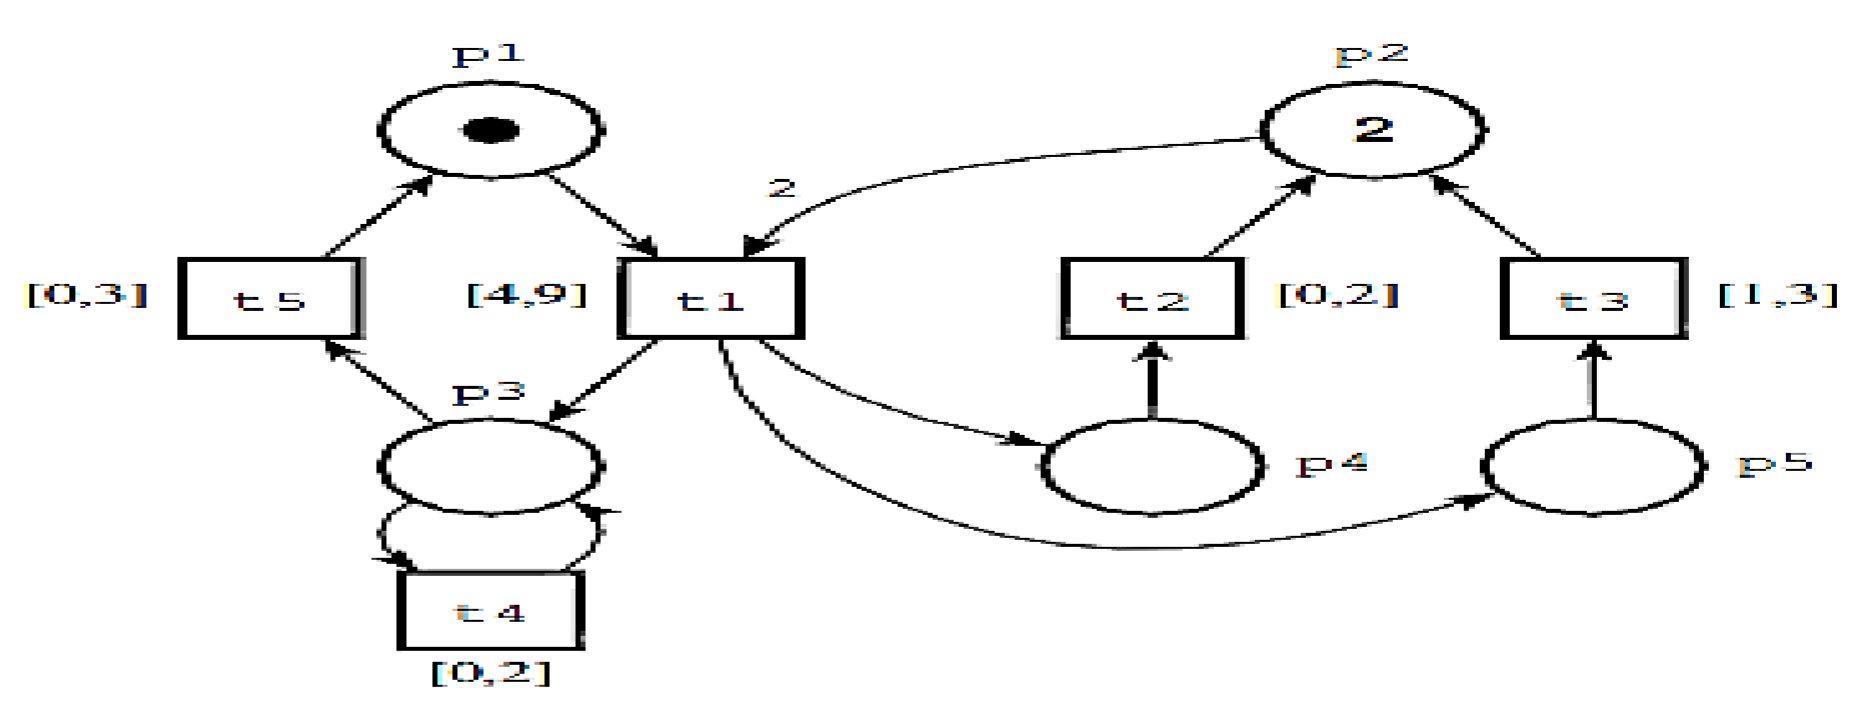
\includegraphics[width=0.7\linewidth]{images/pitrif005}
	\caption{ Exemple de réseau de Pétri temporel }
	\label{fig:pitrif005}
\end{figure}





\section{Réseaux de Petri et workflow
}

Les Réseaux de Petri (RdPs)  constituent un formalisme majeur pour modéliser les processus workflows. Une des forces des RdPs est la base mathématique forte qu'ils offrent avec une représentation graphique. Dans cette section, nous résumons la projection topographique entre concepts de workflow et de RdP  . 

Un processus définit les tâches aussi bien que les conditions pour leur exécution. En utilisant les RdPs, un processus est représenté en conversant sa seule entrée (i.e., un nœud du début) dans une place sans arcs entrants, et sa seule sortie (i.e., nœud de la fin) dans une place sans arcs sortants. Les conditions sont représentées par des places, et les tâches par des transitions. Habituellement, un processus spécifié par RdP devrait accomplir deux exigences : (1) il doit être possible d'accéder à tout moment un état pour lequel il y a un jeton dans la place finale, et (2) quand il y a un jeton dans la place finale, tous les autres jetons auraient dû disparaître.

Dans un processus modélisé par un RdP, une transition active correspond à  un workitem , et le tir d'une transition à une instance de l'activité. Certains work-items peuvent seulement être transformés dans une instance d'activité une fois ils sont déclenchés. Un déclencheur pourrait correspondre à une initiative du participant, à un événement externe ou à un signal du temps initié par l'environnement. A chaque transition correspondante à une tâche qui exige un déclencheur, une autre place d'entrée est ajoutée. Une occurrence du déclencheur apporte un jeton dans cette place supplémentaire. Le jeton est consommé une fois la transition appropriée est franchie. Un échec pendant l'exécution d'une tâche exige un 'rollback' (i.e., revenir à l'état antérieur au début de l'activité). Quand une activité sera complétée avec succès, des changements deviennent définitifs.

\subsection{Modélisation de workflow avec les réseaux de pétri }


Plusieurs recherches ont recommandés l'utilisation des réseaux de pétri pour la modélisation de workflow, et cela à cause de plusieurs facteurs

\subsubsection{Une sémantique formelle } 

Rend la spécification de workflow non ambigüe. L’interprétation de ces spécifications peut être définie mathématiquement.

\subsubsection{Techniques d’analyse} 

Ils existent plusieurs techniques d’analyse de propriétés qualitatives et quantitatives de modèle de workflow à base des réseaux de pétri, une des propriétés qualitatives est de vérifier l’occurrence d’un inter blocage en vérifiant l’accessibilité de toutes les tâches du réseau 

\subsubsection{Expressivité}
Les réseaux de pétri peuvent exprimer la structure des processus ainsi que leurs dynamisme, y compris la concurrence (le parallélisme). Ils servent aussi comme langage pour la définition de la structure d’un processus, simulation de processus et la gestion de workflow


\subsection{Workflow à base de réseaux de pétri (WF-net) }
La modélisation de workflow en terme de réseaux de pétri consiste à modéliser le comportement dynamique du système en représentant les tâches sous forme de transitions, les conditions sous forme de places et les cas sont représentés par les jetons. Les réseaux de pétri qui permettent de modéliser les workflows sont appelés WF-net (réseaux de workflow).

\begin{defn}
\textbf{(Wf-nets):}  Le réseau de pétri qui permet de modéliser le contrôle de flux d’un workflow est appelé un WF-net  (réseaux workflow) Ssi:

\begin{enumerate}
\item Il existe une seule place source $i \in P$ avec $ ^{*}i = \emptyset $ . (i début du processus).

\item  Il existe une seule place puits $o \in P$ avec $ ^{*}o = \emptyset $  (o est la fin du processus).

\item  Chaque nœud $x \in (P \cup T) $est sur un chemin de $i$ à $o$. C’est à dire : Chemin $(i, x)$ $\wedge$ Chemin $(x, o)$.



\end{enumerate} 

\begin{figure}[H]
	\centering
	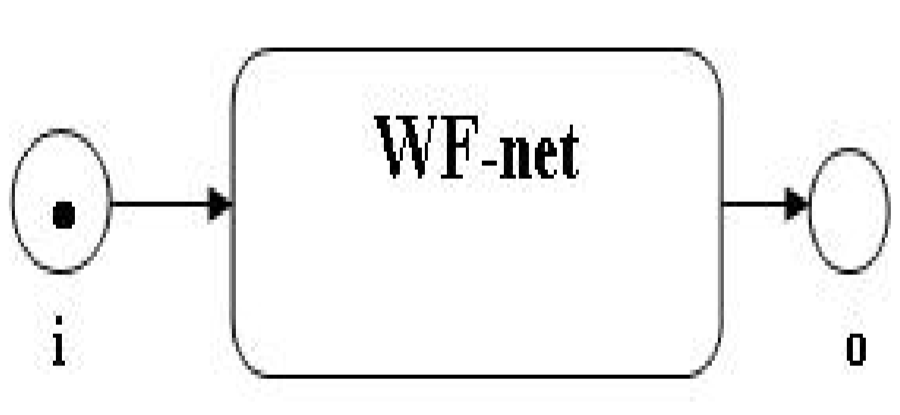
\includegraphics[width=0.5\linewidth]{images/wf-nete006}
	\caption{ Procédure modélisée avec le WF-net }
	\label{fig:wf-nete006}
\end{figure}

\end{defn}
Un réseau de workflow (WF-net) est un réseau de pétri qui possède une seule place d’entrée (i) et une seule place de sortie (o) et puis que n’importe quel cas traité avec la procédure représentée par un WF-net est crée au moment de début de son traitement par le système de gestion de workflow (SGWF) est supprimé une fois que sont traitement est complètement achevé par le SGWF. Cela veut dure que le WFnet spécifie le cycle de vie d’un cas du processus modélisé  .
\begin{rem}
  Un chemin C dans un WF-net d’un nœud $n_{1}$ au nœud $n_{k}$ est une séquence $<n_{1},n_{2},...,n_{k}>$ tel-que $<n_{i},n_{i+1}> \in F $, pour $i=1...k-1$.
  F est la relation de flux. 
\end{rem}

\subsection{Constructions du routage dans un WF-net}
Un réseau de workflow (WF-net) est utilisé pour spécifier le routage de flux dans les cas du workflow, quatre types de routage ont été identifiés :

\subsubsection{Séquentiel :}

Utilisé pour traiter la relation de causalité entre les tâches. Soit deux tâches A et B, si la tâche B et exécutée après l’accomplissement de A, ce comportement peut être modélisé avec un RDP en ajoutant les places pour capter les relations de causalité entre les tâches A et B. La figure \ref{fig:wf003} illustre ce comportement.


\begin{figure}[H]
	\centering
	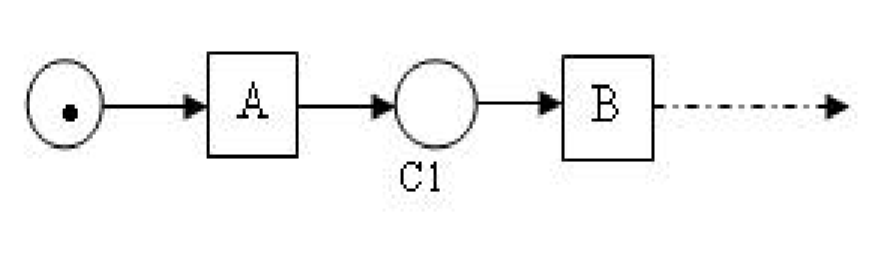
\includegraphics[width=0.7\linewidth]{images/wf003}
	\caption{Routage séquentiel.}
	\label{fig:wf003}
\end{figure}

\subsubsection{Parallèle : }
Utiliser dans le cas où l’ordre d’exécution est moins strict. Par exemple si on a deux tâches B et C qui doivent être exécutées mais dans un ordre arbitraire, la modélisation de ce comportement de routage parallèle comporte deux constructions le AND-split et AND-join.


\begin{figure}[H]
	\centering
	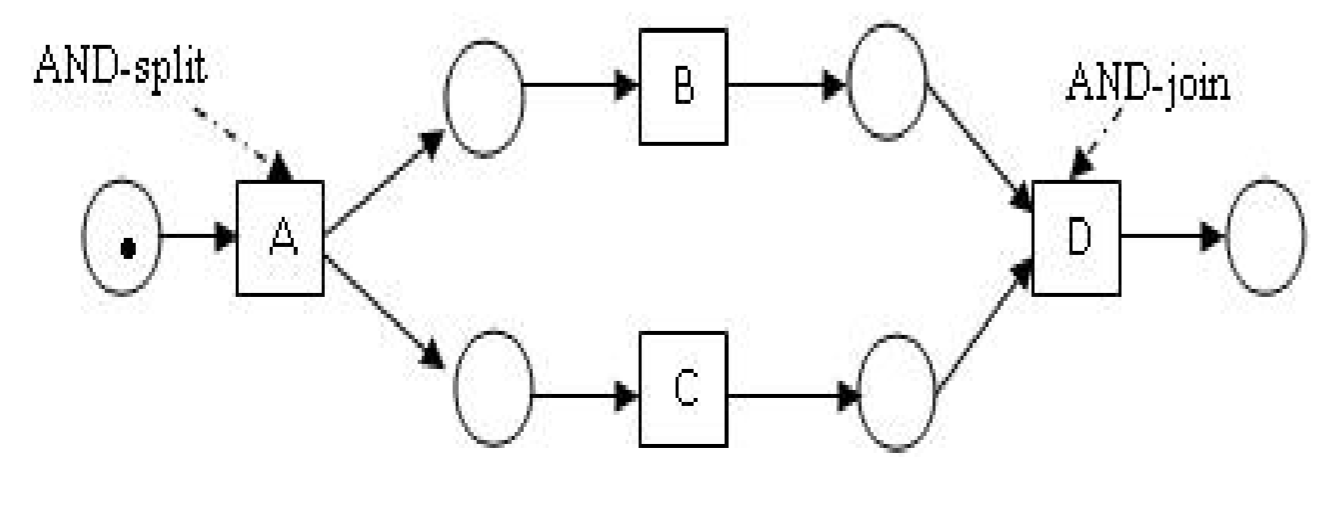
\includegraphics[width=0.7\linewidth]{images/Capture}
	\caption{Routage parallèle.}
	\label{fig:capture}
\end{figure}

\subsubsection{Conditionnel :}

Utilisé pour traiter les cas où le routage de flux peut dépendre des données d’un cas. Il existe deux types de routage conditionnel : \textit{\textbf{le choix non-déterministe}} et \textit{\textbf{le choix déterministe}}. 


\begin{enumerate}

\item \textbf{Choix non-déterministe :} Pour modéliser ce comportement deux constructions sont utilisées OR-Split et OR-join. La figure \ref{fig:wf005} représente un choix entre l’exécution des deux tâches B ou C grâce à un jeton dans la place c2, mais cela permet un choix non-déterministe (l’exécution de B ou de C car les deux tâches sont permises).



\begin{figure}[H]
	\centering
	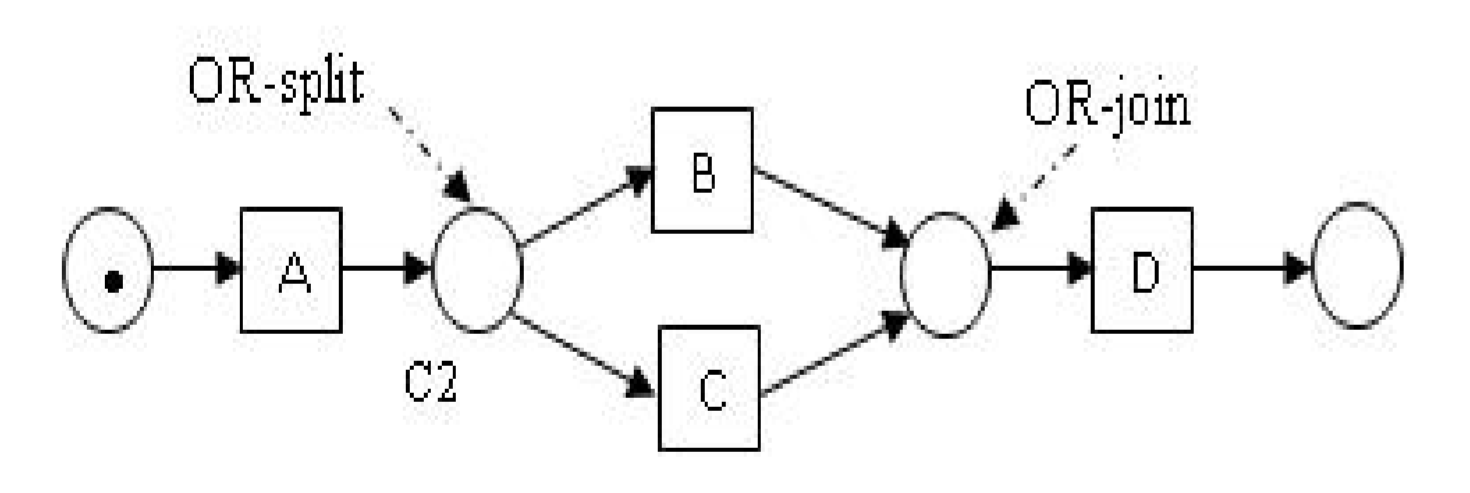
\includegraphics[width=0.7\linewidth]{images/wf005}
	\caption{Routage conditionnel non-déterministe}
	\label{fig:wf005}
\end{figure}



\item \textbf{Choix déterministe : } Le choix entre plusieurs alternatives peut être guidé par les données (ou les attributs) du workflow, dans ce cas c’est un choix déterministe.

Nous pouvons prendre le schéma de la figure précédente et ajouter une pré-condition pour chacune des tâches B et C (en se basant sur un ou plusieurs attributs du workflow).

Il y a une autre façon de modéliser le choix déterministe comme dans la figure suivante. La transition A comporte deux places de sortie c2 et c3 et produit un seul jeton (soit dans c2 ou dans c3). Le choix entre les deux places est basé sur la valeur de l’attribut x.Un symbole spécial est utilisé pour représenté que la tâche A est un OR-split (exclusive OR).
















\end{enumerate}






















\subsection{Techniques et outils de modélisation de workflow}

Associés aux aspects à modéliser définit précédemment, un certain nombre d’outils de modélisation peuvent être employés pour décrire le comportement des flux de travail comme le précise [VAN DER AALST 97a] [VAN DER AALST 97b].

Il existe un certain nombre de techniques de modélisation des procédures, tels que : Pour la représentation en terme de fonctions, les diagrammes de flots de données DFD31, ISAC32, SADT33 semblent tout a fait indiqués.  


Pour l’aspect comportement, les diagrammes état-transition (par extensions : state charts) semblent convenir plus particulièrement. Mais aussi les organigrammes (Flowcharts) qui illustre les pas dans une procédure. En visualisant les procédures, un organigramme peut rapidement aider à identifier des goulots d'étranglement ou des inefficacités dont la procédure peut être rationalisée ou améliorée. 

Concernant l’aspect représentation des données, on pourra utiliser par exemple un Modèle Conceptuel de Données de la méthode MERISE [TARDIEU 85] ou un modèle de classes d’une méthode Objet UML34. Le modèle informationnel peut également représenter le flux des informations, c’est-à-dire leur circulation et les différents états qu’elles peuvent prendre ainsi que les dépendances hiérarchiques.

Il existe également des techniques de diagramme spécifiques aux concepteurs de logiciels utilisées dans les outils de simulation WfMS. Ces outils de modélisation et simulation spécifiques intègrent un outil modélisation, le plus souvent dans un langage graphique et un simulateur également spécifique se basant sur un formalisme particulier après transformation dans ce dit format simulable, par exemple un automate à états finis. 


Mais ce sont certainement les réseaux de Petri de haut niveau qui sont les plus utilisés à l’heure actuelle pour représenter et simuler les comportements des procédures d’un Workflow autour des nombreux travaux de Van der Aalst [VAN DER AALST 98b]. 

Cependant, jusqu’alors pas, ou peu, de travaux de spécification et de modélisation de la partie processus d’un Workflow on été réalisés en utilisant la clarté et la précision du formalisme DEVS. Ce formalisme offre néanmoins un aspect modulaire hiérarchique important dans la définition d’un Workflow. De plus leur simulation par événements discrets permet une exécution rapide. Nous reviendrons sur ce point dans le chapitre 4. 

\subsubsection{Réseaux de Petri et workflow
}
Les Réseaux de Petri (RdPs) \parencite{RdPs} constituent un formalisme majeur pour modéliser les processus workflows. Une des forces des RdPs est la base mathématique forte qu'ils offrent avec une représentation graphique. Dans cette section, nous résumons la projection topographique entre concepts de workflow et de RdP .%[1, 11, 65]. 

Un processus définit les tâches aussi bien que les conditions pour leur exécution. En utilisant les RdPs, un processus est représenté en conversant sa seule entrée (i.e., un nœud du début) dans une place sans arcs entrants, et sa seule sortie (i.e., nœud de la fin) dans une place sans arcs sortants. Les conditions sont représentées par des places, et les tâches par des transitions. Habituellement, un processus spécifié par RdP devrait accomplir deux exigences : (1) il doit être possible d'accéder à tout moment un état pour lequel il y a un jeton dans la place finale, et (2) quand il y a un jeton dans la place finale, tous les autres jetons auraient dû disparaître.

Dans un processus modélisé par un RdP, une transition active correspond à un workitem, et le tir d'une transition à une instance de l'activité. Certains work-items peuvent seulement être transformés dans une instance d'activité une fois ils sont déclenchés. Un déclencheur pourrait correspondre à une initiative du participant, à un événement externe ou à un signal du temps initié par l'environnement. A chaque transition correspondante à une tâche qui exige un déclencheur, une autre place d'entrée est ajoutée. Une occurrence du déclencheur apporte un jeton dans cette place supplémentaire. Le jeton est consommé une fois la transition appropriée est franchie. Un échec pendant l'exécution d'une tâche exige un 'rollback' (i.e., revenir à l'état antérieur au début de l'activité). Quand une activité sera complétée avec succès, des changements deviennent définitifs.

\subsubsection{UML et workflow}


Les diagrammes d'états/transitions sont un autre formalisme majeur pour la modélisation des processus workflows. Ils ont été inventés par Harel \parencite{Harel}, et ont été incorporés dans UML (Unified Modelling Language)  \parencite{UML}, dans une forme légèrement différente. Weissenfels et al. \parencite{EDBT'98} ont investi sur l'usage des diagrammes d'états/transitions pour modéliser les processus workflows (le projet Mentor WfMS). Nous pouvons aussi citer Blake \parencite{WETICE'02} qui a présenté une approche systématique pour la modélisation des workflows en utilisant UML (le projet WARP). 

Dans le projet Mentor WfMS \parencite{EDBT'98}, les activités reflètent la décomposition fonctionnelle d'un système et dénotent les composants actifs d'une spécification; elles correspondent directement aux activités d'un workflow. Un diagramme d'activités spécifie le flot de données entre les activités, dans la forme d'un graphe orienté avec les éléments de données comme annotations des arcs. Les diagrammes d'états capturent le comportement d'un système en spécifiant le flot de contrôle entre les activités.

Pour le projet WARP (Workflow Automation through Agent-based Reflective Processes) \parencite{WETICE'02}, l'approche utilisée distingue entre les vues structurelles, fonctionnelles, non fonctionnelles, et opérationnelles. Les vues structurelles informe sur les activités, la définition des rôles, et la composition du workflow. Elles sont représentées dans UML par les diagrammes des classes. Les vues fonctionnelles montrent le flot de données et de contrôle du workflow en utilisant les diagrammes d'activités UML. Les vues non-fonctionnelles (traitement des erreurs, concurrence, atomicité, etc.) utilisent le flot de données et de contrôle et peuvent être modélisées aussi par les diagrammes d'activités. Finalement, les vues opérationnelles sont reliées à l'initiation des instances du workflow, et la coordination pour l'achèvement du workflow. Ces vues peuvent être modélisées par les diagrammes de séquence UML.

\subsubsection{YAWL}
YAWL (Yet Another Workflow Language) [2] est basé sur les RdPs avec des caractéristiques additionnelles pour faciliter la modélisation des workflows complexes. YAWL hérite de la classe des RdPs et s'étend par la modélisation de l'instance multiple, les tâches composites, le retrait des jetons et les transitions connectées directement.

La spécification du workflow dans YAWL est une sorte de réseaux de workflow étendu (EWF-nets) qui forme une hiérarchie. Une tâche est soit atomique soit composite. Chaque tâche composite fait référence à un unique EWF-net dans le niveau le plus bas de la hiérarchie. Les tâches atomiques forment les feuilles de l'arbre. Il y a un seul EWF-net non référencé par une tâche composite. Cet EWF-net est nommée le niveau le plus haut du workflow et forme la racine. 

Chaque EWF-net consiste en des tâches (composites ou atomiques) et des conditions qui peuvent être interprétées comme des places. 
Chaque EWF-net a une unique condition d'entrée et une unique condition de sortie. Contrairement aux RdPs, il est possible de connecter les transitions. Sémantiquement, cette construction peut être interprétée comme une condition ignorée.

Chaque tâche peut avoir des instances multiples. Nous pouvons créer un seuil maximal et un seuil minimal pour le nombre d'instances après l'initiation d'une tâche. En plus, il est possible d'indiquer que la tâche se termine au moment ou certaines instances seuils sont achevées

\section{Les réseaux de Petri}

Les réseaux de Petri(Petri,1962)sont une généralisation des automates a états. Ils offrent un contexte général pour modéliser la concurrence et la synchronisation dans les systèmes distribués. Un réseau de Petri est un graphe biparti alterné qui possède deux types de nœuds: les places(cercles)et les transitions(rectangles). Des arcs(flèches) relient les places aux transitions(figure \ref{fig:2 rdp}). L'état du système,nommé marquage,est défini par la répartition des jetons dans les places. Une transition est franchissable sous certaines conditions, notamment lorsqu'il y a suffisamment de jetons dans ses places d’entrée. Le franchissement d’une transition se traduit par une modification du marquage consistant en la consommation des jetons indispensables au franchissement de la transition et la création éventuelle de nouveaux jetons dans les places en sortie de la transition.
\begin{figure}[h]
	\centering
	
	\begin{subfigure}[b]{0.3\textwidth}
		\centering
		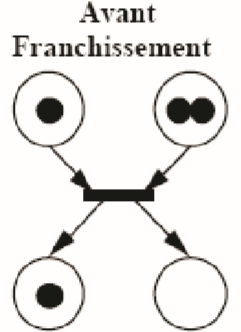
\includegraphics[width=\textwidth]{petrif1}
		\caption{$M_{t}=(1,2,1,0)$}
		\label{fig:three sin x}
	\end{subfigure}
	\hfill
	\begin{subfigure}[b]{0.3\textwidth}
		\centering
		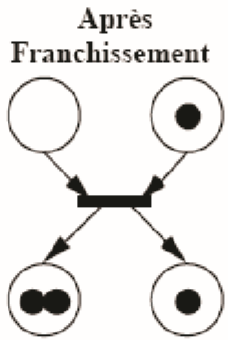
\includegraphics[width=\textwidth]{pitrif2}
		\caption{$M_{t+1}=(0,1,2,1)$}
		\label{fig:five over x}
	\end{subfigure}
	
	\caption{Opération de franchissement}
	\label{fig:2 rdp}
\end{figure}

\subsection{Définition}

\begin{defn}\textbf{\textbf{(Réseau de Petri simple):}}
	\\
Un réseau de Petri simple est un tuple
 (P,T,Pre,Post,M0):
 
 \begin{itemize}
\item  	P est un ensemble final de places,
\item T est un ensemble final de transition $ (P \cap T = \theta ) $ ,
\item Pre: $P \times T \to N$ est la fonction d'incidence avant,
\item Post: $P \times T \to N$ est la fonction d'incidence arriére,
\item $M_{0}$ et le marquage initial $M_{0}:  P \to N$.
  \end{itemize}

\end{defn}




Un réseau de Petri peut-être evucommeun système de transitions dont les états sont les marquages du réseau et les transitions entre états correspondent au franchissement des transitions du réseau.




\section{Modélisation Des Politiques De Sécurité}

Durant les dernières années, l'utilisation des réseaux de Petri s'est répandue grâce au nombre de travaux qui a été développé pour enrichir les réseaux de Petri ainsi que la disponibilité des outils. Selon de nombreux chercheurs (Osborn, 2002), les réseaux de Petri sont le seul formalisme qui permet de modéliser la structure du système et de faire des analyses qualitative et quantitative. Les réseaux de Petri ont été utilisés pour la vérification de la sécurité(Ahmed and Tripathi,2003),pour la spécification des autorisations dans les workflows \parencite{ESORICS'96},l'analyse des politiques de sécurité y compris les politiques de contrôle d'accès discrétionnaires (Kumaretal. ,2002; Knorr, 2000), mandataires(Knorr, 2001; Varadharajan, 1991; Juopperi, 1995; Juszczyszyn, 2003; Jiangetal., 2004; Rakkay and Boucheneb, 2006; Zhangetal., 2006b; Zhangetal., 2006a) et à base de ro les(Koch et al.,2002;Rakkay and Boucheneb, 2007;Shafiq et al.,2005).

 














